\documentclass{article}
\usepackage[utf8]{inputenc}
\usepackage{graphicx}

\title{Chapter 1}
\author{Ilham Dwi Prasetyo Nugroho}
\date{March 2021}

\begin{document}

\maketitle


\section{Teori}
\subsection{Definisi Kecerdasan Buatan}
\hfill\break
sebuah keilmuan yang didapat dari pemikiran manusia dalam bentuk pemberian informasi jadi terbentuklah teknologi computer yang kian berkembang

\subsection{Sejarah dan Perkembangan Kercerdasan Buatan}
\hfill\break
Istilah AI pertama kali dikemukakan pada tahun 1956 dikonferensi Darthmouth. Sejak saat itu AI terus dikembangkan sebab berbagai penelitian mengenai teori-teori dan prinsip-prinsipnya juga terus berkembang. Meskipun istilah AI baru muncul tahun 1956, tetapi teori-teori mengarah ke AI sudah muncul sejak tahun 1941. Berikut ini tahapan-tahapan sejarah perkembangan AI:
\begin{enumerate}
	\item Era Komputer Elektronik (1941)
	\hfill\break
	Pada tahun 1941 telah ditemukan alat penyimpanan dan pemrosesan informasi. Penemuan tersebut dinamakan komputer elektronik yang dikembangkan di USA dan Jerman. Komputer pertama ini memerlukan ruangan yang luas dan ruang AC yang terpisah. Saat itu komputer meibatkan konfigurasi ribuan kabel untuk menjalankan suatu program. Hal ini sangat merepotkan bagi para programmer. Pada tahun 1949, berhasil dibuat komputer yang mampu menyimpan program sehingga membuat pekerjaan untuk memasukkan program menjadi lebih mudah. Penemuan ini menjadi dasar pengembangan program yang mengarah ke AI.

	\item Masa Persiapan AI (1943–1956)
	\hfill\break
	Pada tahun 1943, Warren McCulloch dan Walter Pitts mengemukakan tiga hal: pengetahuan fisiologi dasar dan fungsi sel syaraf dalam otak, analisis formal tentang logika proporsi (propositional logic), dan teori komputasi turing. Mereka berhasil membuat suatu model syaraf tiruan (artificial neuron) di mana setiap neuron digambarkan sebagai on dan off. Mereka menunjukkan bahwa setiap fungsi dapat dihitung dengan suatu jaringan sel syaraf dan bahwa semua hubungan logis dapat diimplementasikan dengan struktur jaringan yang sederhana.
	\noindent
	Pada tahun 1950, Norbert Wiener mebuat penelitian mengenai prinsip-prinsip teori feedback. Contoh yang terkenal adalah thermostat. Penemuan ini juga merupakan awal perkembangan AI. Pada tahun 1956, John McCarthy (yang setelah lulus dari Princeton kemudian melanjutkan ke Dartmouth College) meyakinkan Minsky, Claude Shannon dan Nathaniel Rochester untuk membantunya melakukan penelitian dalam bidang Automata, jaringan sel syaraf dan pembelajaran intelejensia. Mereka mengerjakan proyek ini selama dua bulan di Dartmouth. Hasilnya adalah program yang mampu ber-pikir non-numerik dan menyelesaikan masalah pemikiran, yang dinamakan Principia Mathematica. Hal ini menjadikan McCarthy disebut sebagai Father of AI (Bapak AI).

	\item Awal Perkembangan AI (1952–1969)
	\hfill\break
	Pada tahun-tahun pertama pengembangannya, AI mengalami banyak kesuksesan. Diawali dengan kesuksesan Newell dan Simon dengan sebuah program yang disebut General Problem Solver. Program ini dirancang untuk memulai penyelesaian masalah secara manusiawi. Pada tahun 1958, McCarthy di MTT Lab Memo No. 1 mendefinisikan bahasa pemrograman tingkat tinggi yaitu LISP, yang sekarang mendominasi pembuatan program-program AI. Kemudian, McCarthy membuat program yang dinamakan Programs With Common Sense. Di dalam program tersebut, dibuat rancangan untuk menggunakan pengetahuan dalam mencari solusi. Pada tahun 1959, Nathaniel Rochester dari IBM dan mahasiswa-mahasiswanya mengeluarkan program AI Geometry Theorm Prover. Program ini dapat membuktikan suatu teorema menggunakan axioma-axioma yang ada. Pada tahun 1963, program yang dibuat James Slagle mampu menyelesaikan masalah integral tertutup untuk mata kuliah kalkulus. Pada tahun 1968, program analogi buatan Tom Evan menyelesaikan masalah analogi geometris yang ada pada tes IQ.

	\item Perkembangan AI Melambat (1966–1974)
	\hfill\break
	Prediksi Herbert Simon pada tahun 1957 yang menyatakan bahwa AI akan menjadi ilmu pengetahuan yang akan berkembang dengan pesat ternyata meleset. Pada 10 tahun kemudian, perkembangan AI melambat. Hal ini disebabkan adanya 3 kesulitan utama yang dihadapi AI, yaitu:
	\begin{enumerate}
		\item Masalah pertama: program-program AI yang bermunculan hanya mangandung sedikit atau bahkan tidak mengandung sama sekali pengetahuan (knowledge) pada subjeknya. Program-program AI berhasil hanya karena manipulasi sintetis yang sederhana. Sebagai contoh adalah Weizenbaum’s ELIZA program (1965) yang dapat melakukan percakapan serius pada berbagai topik, sebenarnya hanyalah peminjaman dan manipulasi kalimat-kalimat yang diketikkan oleh manusia.
		\item Masalah kedua: banyak masalah yang harus diselesaikan oleh AI. Karena terlalu banyaknya masalah yang berkaitan, maka tidak jarang banyak terjadi kegagalan pada pembuatan program AI.
		\item Masalah ketiga: ada beberapa batasan pada struktur dasar yang digunakan untuk menghasilkan perilaku intelejensia. Sebagai contoh adalah pada tahun 1969 buku Minsky dan Papert Perceptrons membuktikan bahwa program-program perceptrons dapat mempelajari segala sesuatu, tetapi program-program tersebut hanya mempresentasikan sejumlah kecil saja. Sebagai contoh dua masukan perceptrons yang berbeda tidak dapat dilatihkan untuk mengenali kedua masukan yang berbeda tersebut.
	\end{enumerate}

	\item Sistem Berbasis Pengetahuan (1969–1979)
	\hfill\break
	Pengetahuan adalah kekuatan pendukung AI. Hal ini dibuktiikan dengan program yang dibuat oleh Ed Feigenbaum,Bruce Buchanan dan Joshua Lederberg yang membuat program untuk memecahkan masalah struktur molekul dari informasi yang didapatkan dari spectometer massa. Program ini dinamakan Dendral programs yang berfokus pada segi pengetahuan kimia. Dari segi diagnosis media juga sudah ada yang menemukannya, yaitu Saul Amarel dalam proyek computer in biomedicine. Proyek ini diawali dari keinginan untuk mendapatkan diagnosa penyakit berdasarkan pengetahuan yang ada pada mekanisme penyebab proses penyakit.

	\item AI Menjadi Sebuah Industri (1980–1988)
	\hfill\break
	Industrialisasi AI diawali dengan ditemukannya expert system (sistem pakar) yang dinamakan R1 yang mampu mengkonfigurasi sistem-sistem komputer baru. Program tersebut mulai dioperasikan di Digital Equipment Corporation(DEC), McDermott, pada tahun 1982. Pada tahun 1986, program ini telah berhasil menghemat US\$40 juta per tahun. Pada tahun 1988, kelompok AI di DEC menjalankan 40 sistem pakar. Hampir semua perusahaan besar di USA mempunyai divisi AI sendiri yang menggunakan ataupun mempelajari sistem pakar. Booming industri AI ini juga melibatkan perusahaan-perusahaan besar seperti Carnegie Group, Inference, Intellicorp, dan Technoledge yang menawarkan software tools untuk membangun sistem pakar. Perusahaan hardware seperti LISP dan Machines Inc., Texas Instruments, Symbolics, dan Xerox juga turut berperan dalam membangun workstation yang dioptimasi untuk pembangunan program LISP. Sehingga, perusahaan yang sejak tahun 1982 hanya menghasilkan beberapa juta US dolar per tahun meningkat menjadi 2 milyar US dolar per tahun pada tahun 1988.

	\item Kembalinya Jaringan Syaraf Tiruan (1986–Sekarang)
	\hfill\break
	Meskipun bidang ilmu komputer menolak jaringan syaraf tiruan setelah diterbitkannya buku "perceptrons" karangan Minsky dan Papert, tetapi para ilmuan masih mempelajari bidang ilmu tersebut dari sudut pandang yang lain yaitu fisika. Para ahli seperti Hopfield (1982) menggunakan teknik-teknik mekanika statistika untuk menganalisa sifat-sifat penyimpanan dan optimasi pada jaringan syaraf. Para ahli psikollogi, David Rumelhart dan Geoff Hinton, melanjutkan penelitian mengenai model syaraf pada memori. Pada tahun 1985-an sedikitnya empat kelompok riset menemukan kembali algoritma belajar propagasi balik (Back-Propagation Learning). Algoritma ini berhasil diimplementasikan kedalam bidang ilmu komputer dan psikologi.

\end{enumerate}
\subsection{Supervised Learning}
\hfill\break
Merupakan data yang dilengkapi dengan tambahan atribut yang ingin kami prediksi
\subsection{Klasifikasi}
\hfill\break Klasifikasi adalah pengelompokan data dimana data yang digunakan memiliki label atau kategori sasaran. Oleh karena itu, algoritma yang digunakan untuk menyelesaikan masalah klasifikasi dapat dibagi menjadi supervised learning atau supervised learning
\subsection{regresi}
\hfill/brea kregresi Merupakan metode statistik yang digunakan di bidang keuangan, investasi dan disiplin ilmu lainnya. Kuncinya adalah menentukan kekuatan dan karakteristik hubungan antara variabel dependen (biasanya diwakili oleh Y) dan serangkaian variabel lain (disebut variabel independen).
\subsection{Unsupervised learning}
\hfill\break Unsupervisedlearning merupakan Algoritme pembelajaran yang digunakan untuk menarik kesimpulan dari kumpulan data. cara ini hanya mempelajari data berdasarkan kedekatannya atau biasa disebut clustering. Metode pembelajaran tanpa pengawasan yang paling umum adalah analisis cluster, yang digunakan dalam analisis data untuk menemukan pola atau pengelompokan tersembunyi dalam data

\subsection{Data set}
\hfill\break Dalam data mining, data masukan data yang akan diolah disebut juga data set. Kumpulan data merupakan kumpulan dari objek data atau biasa disebut catatan, titik, vektor, pola, kejadian, pengamatan, kasus atau bahkan data
\subsection{training set}
\hfill\break Training set adalah bagian dari kumpulan data yang kami latih untuk membuat prediksi atau menjalankan fungsi algoritme ML.

\section{Instalasi}
\subsection{Praktek}
\begin{enumerate}
	\item Instalasi Library scikit dari Anaconda, mencoba kompilasi dan uji coba ambil contoh kode dan lihat variabel explorer
	\hfill\break
	\begin{figure}[h]
		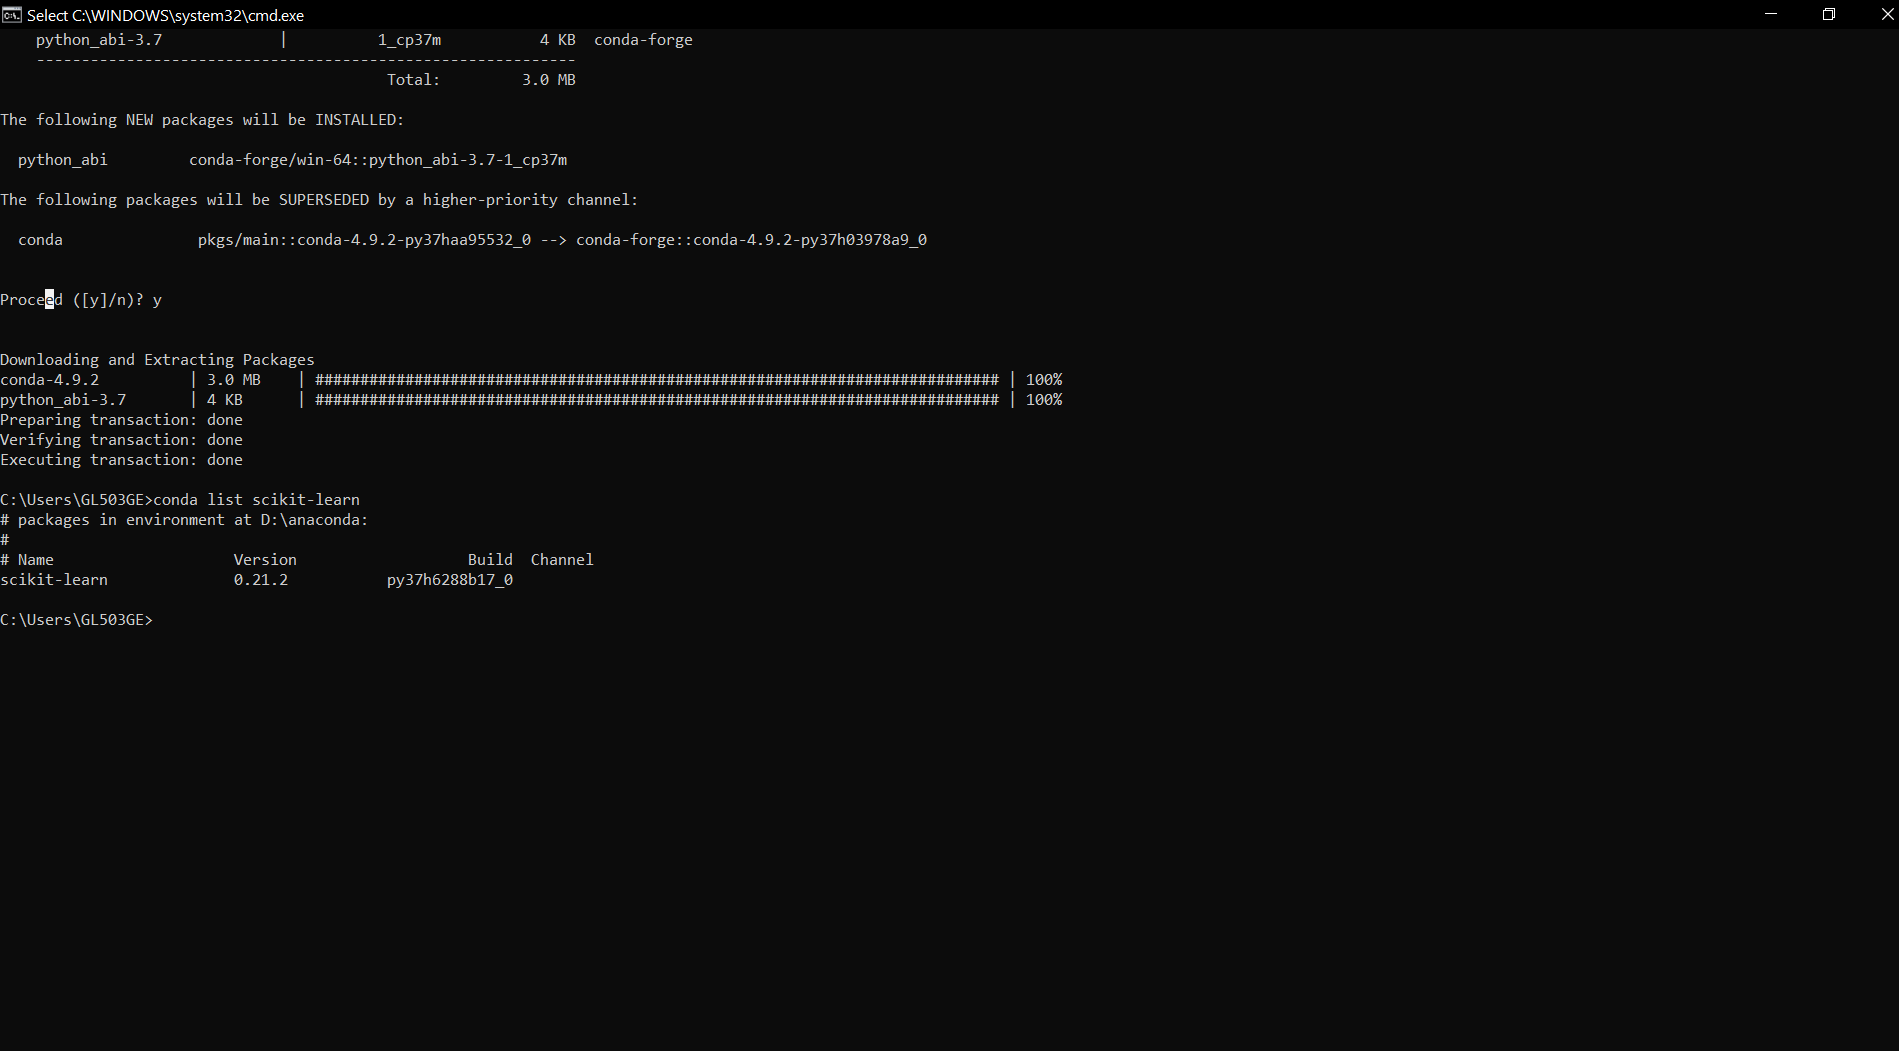
\includegraphics[width=10cm]{figures/1184057/chapter1/Hasil1.png}
		\centering
		\caption{Instalasi Library Scikit Learn}
	\end{figure}
	\newpage\item Uji coba loading an example dataset
	\hfill\break
\lstinputlisting[firstline=7, lastline=18]{src/1184077/chapter1/Tugas1.py}
\item Uji coba Learning dan predicting
	\hfill\break
	\lstinputlisting[firstline=19, lastline=34]{src/1184077/chapter1/Tugas1.py}
\item Uji coba Model Persistence
	\hfill\break
	\lstinputlisting[firstline=37, lastline=64]{src/1184077/chapter1/Tugas1.py}	
	\item Uji coba Conventions
	\hfill\break
	\lstinputlisting[firstline=65, lastline=86]{src/1184077/chapter1/Tugas1.py}
	\end{enumerate}


\section{Penanganan Error}
\begin{enumerate}
\item ScreenShoot Error
	\begin{figure}[h]
		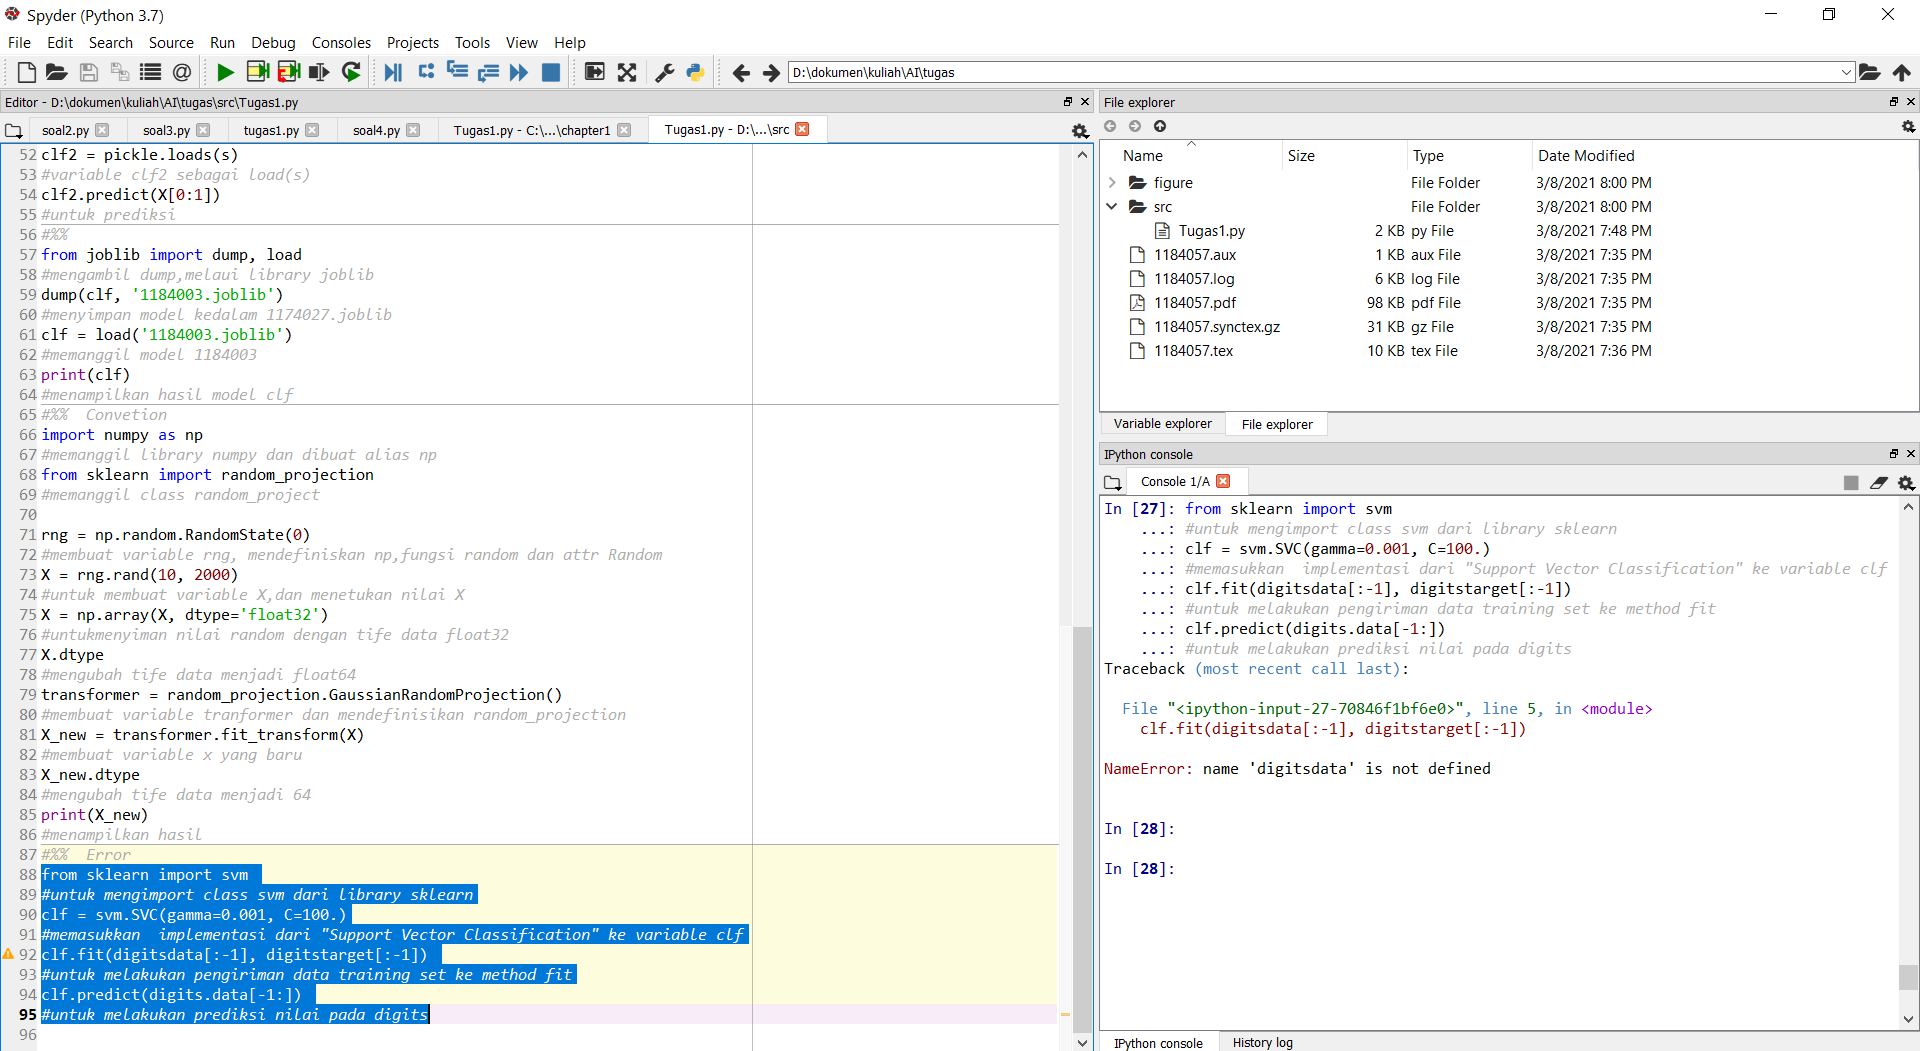
\includegraphics[width=10cm]{figures/1184057/chapter1/Error.PNG}
		\centering
		\caption{Name Error}
	\end{figure}
	\newpage\item Tuliskan Kode Error dan Jenis Error
	\hfill\break
	\lstinputlisting[firstline=87, lastline=9]{src/1184077/chapter1/Tugas1.py}
\hfill\break
	\item Cara Penangan Error
\hfill\break Tambahkan prediksi nilainya agar kode program dapat terbaca
	\end{enumerate}
\section{Bukti Tidak Plagiat}
\begin{figure}[h]it
	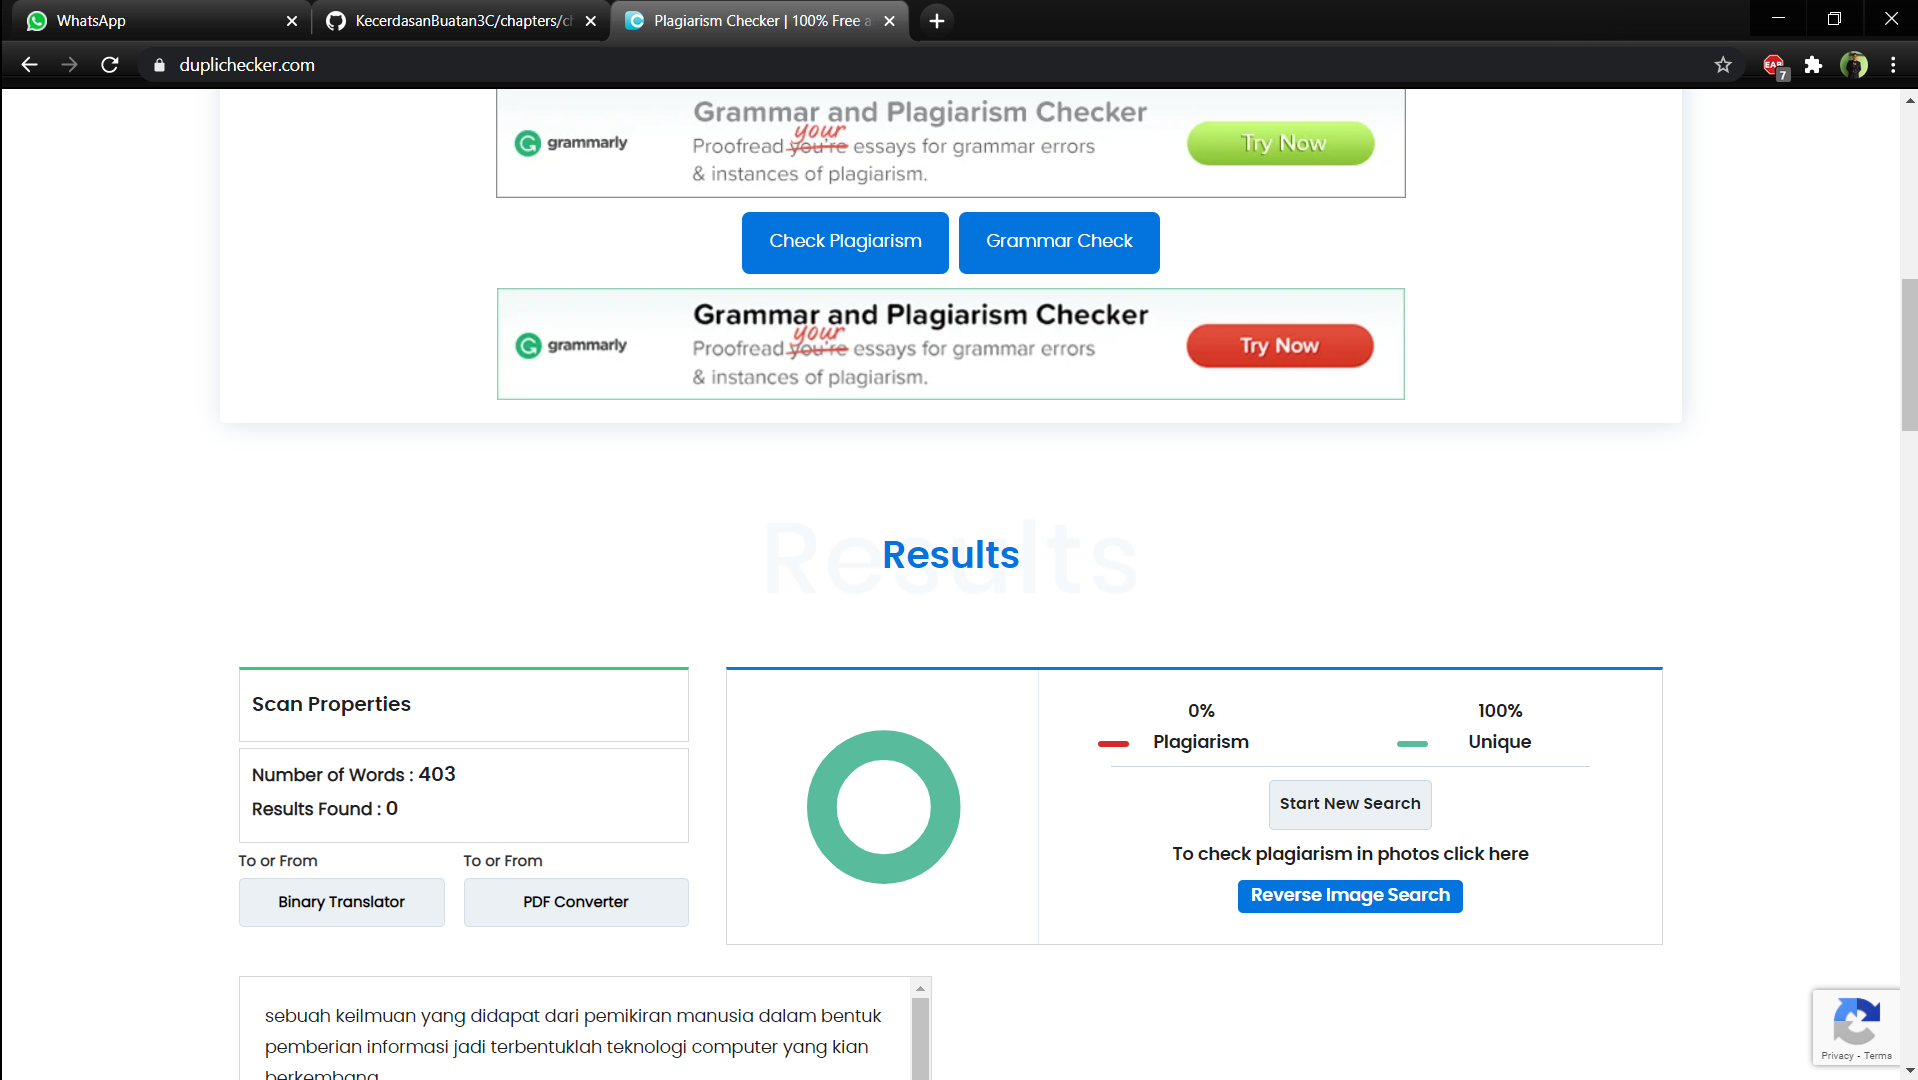
\includegraphics[width=10cm]{figures/1184057/chapter1/Plagiat.png}
	\centering
	\caption{Bukti Tidak Melakukan Plagiat Chapter 1}
	\end{figure}

\end{document}
